\documentclass[answers]{exam}

%% Language and font encodings
\usepackage[english]{babel}
\usepackage[utf8x]{inputenc}
\usepackage[T1]{fontenc}
% \usepackage{enumitem}
%% Sets page size and margins
\usepackage[a4paper,margin=2cm]{geometry}

%% Useful packages
\usepackage{amsmath}
\usepackage{amssymb}
\usepackage{graphicx}
\usepackage{paralist}
\usepackage{framed}
\usepackage{tikz}
\usepackage{float}
\usepackage{listings}
\usepackage{xcolor}
\usepackage{subfigure}
\tikzset{
  % define the bar graph element
  bar/.pic={
    \fill (-.1,0) rectangle (.1,#1) (0,#1) node[above,scale=1/2]{$#1$};
  }
}
\definecolor{codegreen}{rgb}{0,0.6,0}
\definecolor{codegray}{rgb}{0.5,0.5,0.5}
\definecolor{codepurple}{rgb}{0.58,0,0.82}
\definecolor{backcolour}{rgb}{0.95,0.95,0.92}
% Colored Python listing from https://www.overleaf.com/learn/latex/Code_listing
\definecolor{codegreen}{rgb}{0,0.6,0}
\definecolor{codegray}{rgb}{0.5,0.5,0.5}
\definecolor{codepurple}{rgb}{0.58,0,0.82}
\definecolor{backcolour}{rgb}{0.95,0.95,0.92}
 
\lstdefinestyle{mystyle}{
    backgroundcolor=\color{backcolour},   
    commentstyle=\color{codegreen},
    keywordstyle=\color{magenta},
    numberstyle=\tiny\color{codegray},
    stringstyle=\color{codepurple},
    basicstyle=\ttfamily\footnotesize,
    breakatwhitespace=false,         
    breaklines=true,                 
    captionpos=b,                    
    keepspaces=true,                 
    numbers=left,                    
    numbersep=5pt,                  
    showspaces=false,                
    showstringspaces=false,
    showtabs=false,                  
    tabsize=2
}
\lstset{style=mystyle}

\usetikzlibrary{matrix}

\setlength\FrameSep{4pt}
\title{Probability \& Statistics\\ Project}
\author{Hana Ali Rashid, hr05940\\ Tasmiya Malik, Student ID\\ Ifrah Ilyas, Student ID}
\date{\today{}}
\begin{document}
\maketitle


\section*{Q1: Random Walk}
\subsection*{1.1}
In order to simulate a random walk, the following function takes in values of $n$ (number of steps to take), and $p$ (the probability of the object moving one step to the right). It then generates a random number and uses the given probability to determine the direction that the object moves in, and returns the final position.
\lstinputlisting[firstline=5,lastline=13,language=python]{q1.py}
The following function uses the \texttt{get\_updated\_position()} function to get 25 outcomes which are then used to calculate a single expected value for the final position. This is repeated 50 times and the histogram of all these expected values is then plotted.
\lstinputlisting[firstline=16,lastline=31,language=python]{q1.py}
\pagebreak

\begin{figure}
  \centering
  \mbox{\subfigure[No. of steps taken = 10 with probability of moving a step right = 0.5.]{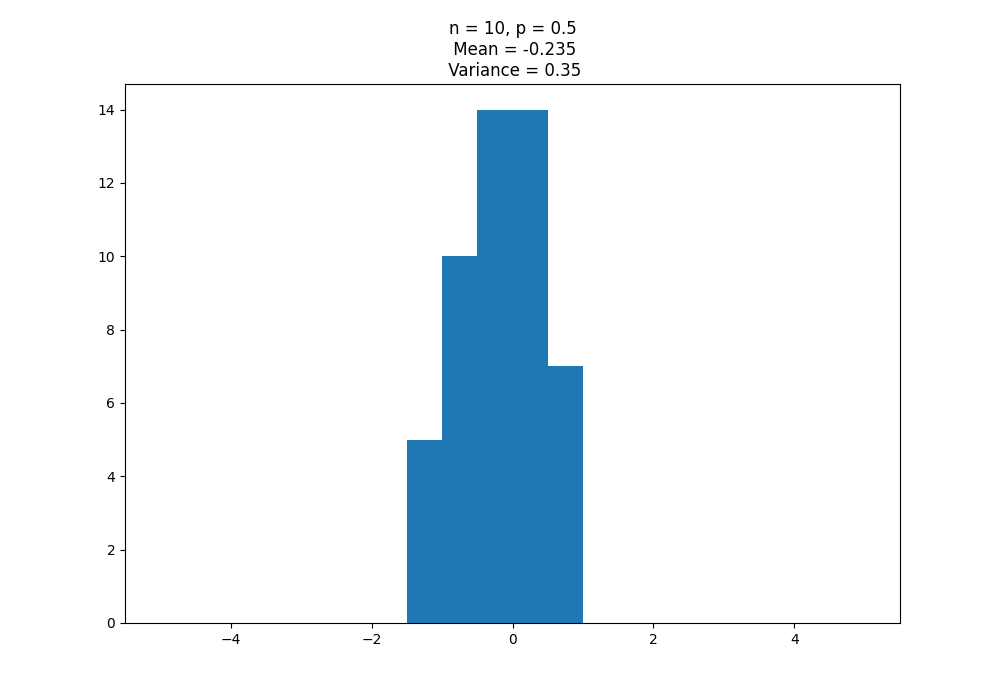
\includegraphics[scale = 0.35]{Q1_histograms/1.1/q1_n = 10_ p = 0.5.png}}\quad
  \subfigure[No. of steps taken = 18 with probability of moving a step right = 0.5.]{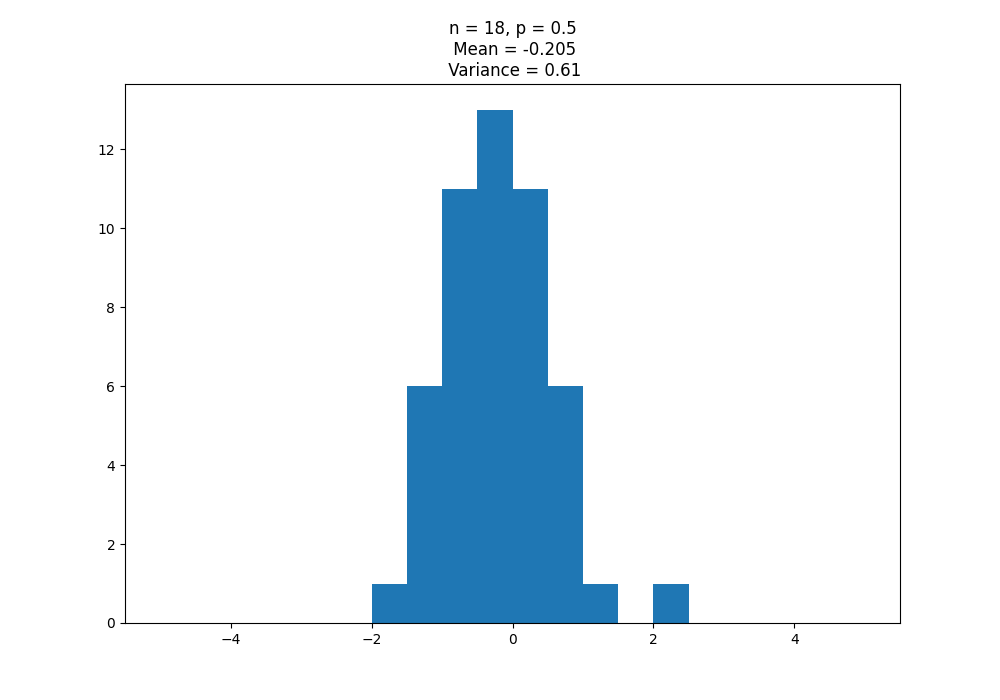
\includegraphics[scale = 0.35]{Q1_histograms/1.1/q1_n = 18_ p = 0.5.png} }}
\end{figure}
\begin{figure}
  \centering
  \mbox{\subfigure[No. of steps taken = 10 with probability of moving a step right = 0.7.]{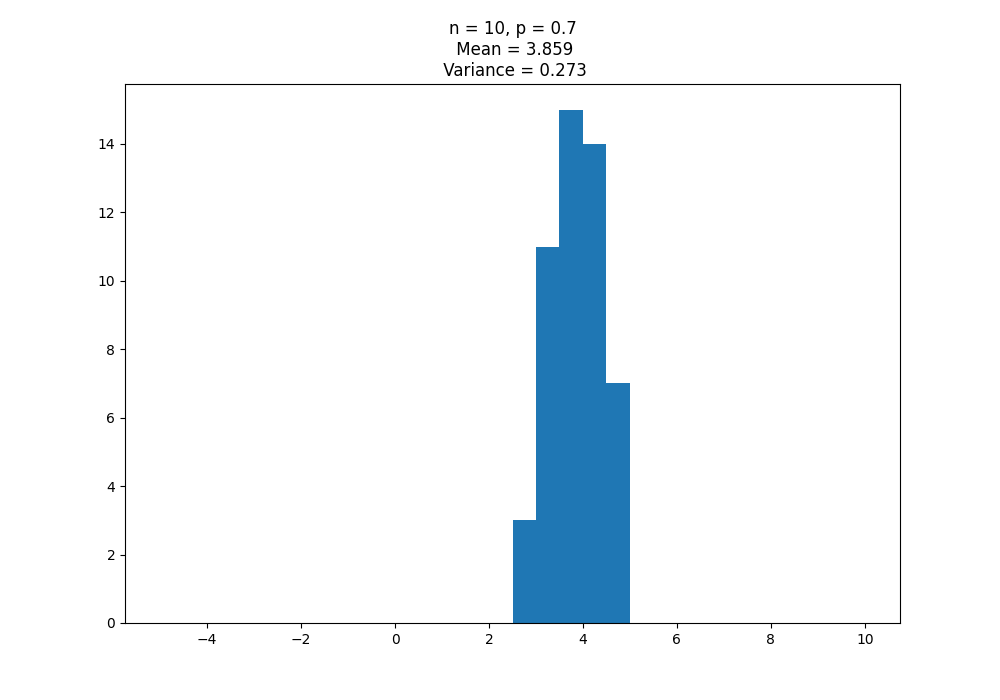
\includegraphics[scale = 0.4]{Q1_histograms/1.1/q1_n = 10_ p = 0.7.png}}}
\end{figure}

Histograms produced by the above code for expected final positions of objects against frequency, where $n$ is the number of steps taken and $p$ is the probability of the object moving one step to the right.\\
\\
Histograms $(a)$ and $(b)$ have the same value of $p$ and varying number of steps $n$. \\
Both histograms appear to follow a normal distribution, with $(a)$ having a mean of $-0.235$ and a variance of $0.35$ and $(b)$ having a mean of $-0.205$ and a variance of $0.61$. Increasing the number of steps has not had a significant effect on the mean but did increase the variance.\\ \\
Histograms $(a)$ and $(c)$ have the same number of steps $n$ and varying values of $p$. \\
Histogram $(c)$ also appears to follow a normal distribution, having a mean of $3.859$ and a variance of $0.273$. Increasing $p$ appears to have affected the mean of the distribution but not the variance as such.\\


\pagebreak
%--------------------------------  1.2  ------------------------------------
\subsection*{1.2}
The following function is the modified version of the \texttt{get\_updated\_position()} function from the previous part such that the object cannot move into the negative part of the number line.
\lstinputlisting[firstline=34,lastline=42,language=python]{q1.py}
The following function uses the \texttt{get\_updated\_position\_restricted()} function to get 25 outcomes which are then used to calculate a single expected value for the final position. This is repeated 50 times and the histogram of all these expected values is then plotted.
\lstinputlisting[firstline=44,lastline=59,language=python]{q1.py}
\pagebreak

\begin{figure}
  \centering
  \mbox{\subfigure[No. of steps taken = 20 with probability of moving a step right = 0.5.]{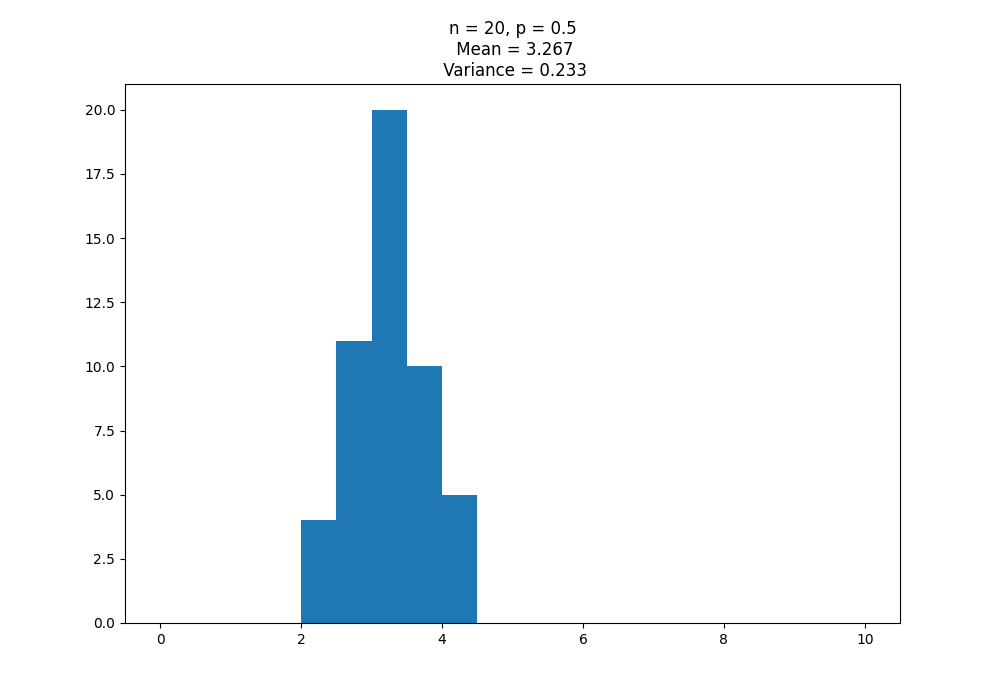
\includegraphics[scale = 0.35]{Q1_histograms/1.2/Q1.2 _n = 20_p = 0.5.png}}\quad
  \subfigure[No. of steps taken = 24 with probability of moving a step right = 0.5.]{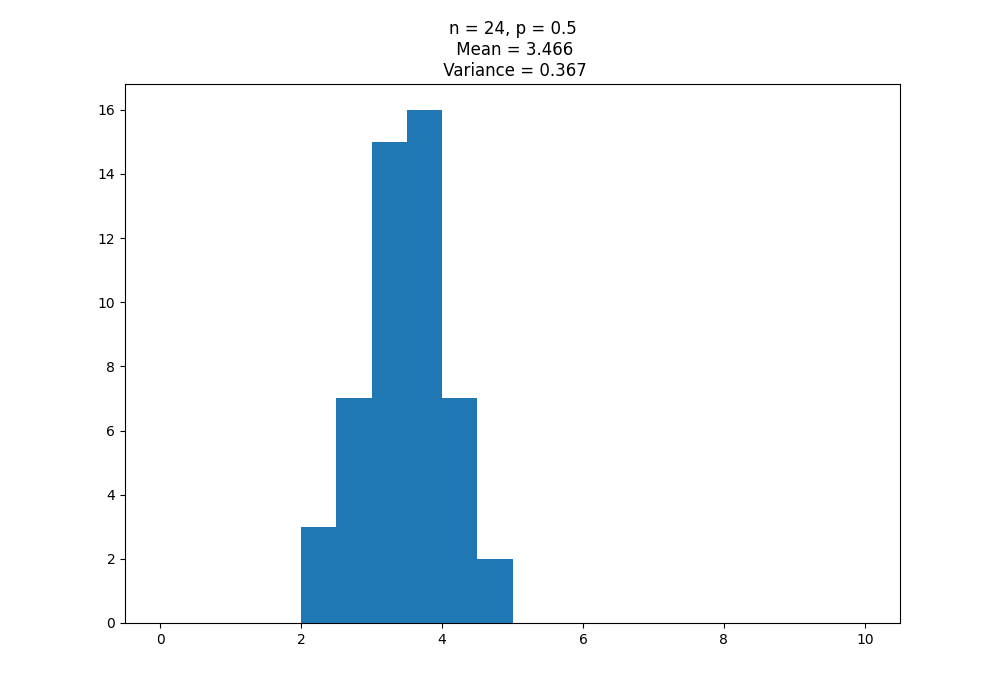
\includegraphics[scale = 0.35]{Q1_histograms/1.2/Q1.2 _n = 24_p = 0.5.png}}}
\end{figure}
\begin{figure}
  \centering
  \mbox{\subfigure[No. of steps taken = 20 with probability of moving a step right = 0.7.]{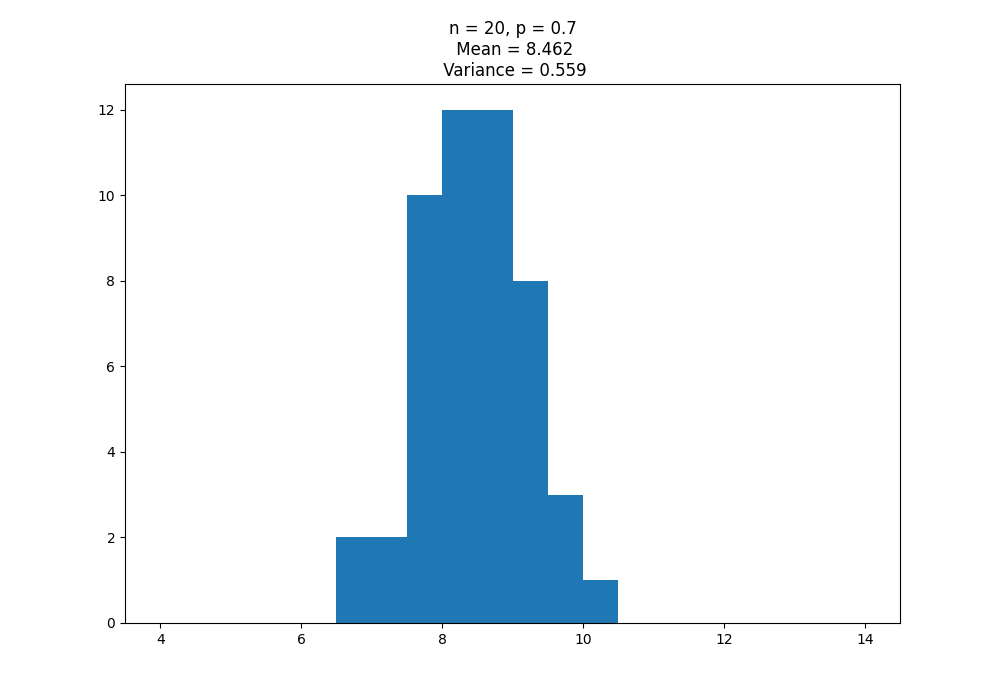
\includegraphics[scale = 0.35]{Q1_histograms/1.2/Q1.2 _n = 20_p = 0.7.png}}\quad
  \subfigure[No. of steps taken = 24 with probability of moving a step right = 0.7.]{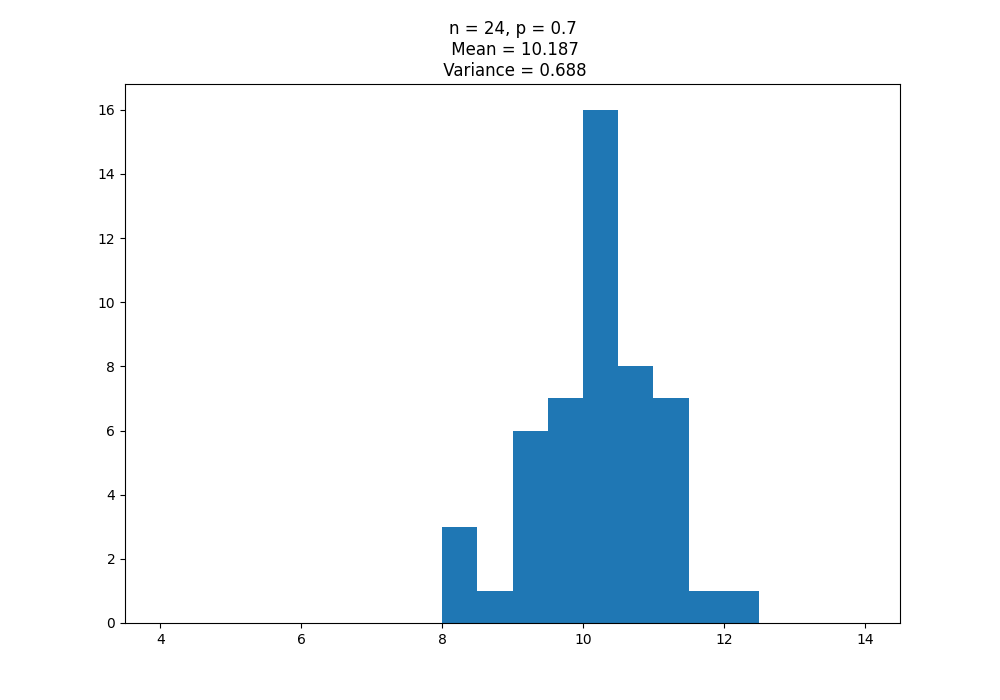
\includegraphics[scale = 0.35]{Q1_histograms/1.2/Q1.2 _n = 24_p = 0.7.png}}}
\end{figure}

Histograms produced by the above code for expected final positions of objects against frequency, where $n$ is the number of steps taken and $p$ is the probability of the object moving one step to the right.\\
\\
Histograms $(d)$ and $(e)$ have the same value of $p$ and varying number of steps $n$. \\
Both histograms appear to follow a normal distribution, with $(d)$ having a mean of $3.267$ and a variance of $0.233$ and $(e)$ having a mean of $3.466$ and a variance of $0.367$. Again, increasing the number of steps has not had a significant effect on the mean but did increase the variance.\\ \\
Histograms $(f)$ and $(g)$ have the same number of steps $n$ respectively as $(d)$ and $(e)$ and varying values of $p$. 
They also appear to follow a normal distribution, with $(f)$ having a mean of $8.462$ and a variance of $0.559$ and $(g)$ having a mean of $10.187$ and a variance of $0.668$. Increasing $p$ appears to have increased the mean and variance, but the mean has increased more significantly. \\ \\
Additionally, due to the added constraint in this part, we see that no expected value for the final position is negative.

\pagebreak
%--------------------------------  1.3  ------------------------------------
\subsection*{1.3}
In this part, we are required to find the number of steps taken by two objects initialized at different points, and moving randomly to meet. The following function takes in the initial position of both objects $pos1$ and $pos2$ as well as their probabilities $p1$ and $p2$, generates random numbers and determines the number of steps taken to meet.
\lstinputlisting[firstline=61,lastline=75,language=python]{q1.py}
The following function uses the \texttt{stepsToMeet} function and calculates 25 expected values using 25 outcomes based on the values of $pos1, pos2, p1$ and $p2$. It then plots a histogram of these expected values as well.
\lstinputlisting[firstline=77,lastline=97,language=python]{q1.py}
\pagebreak
Histograms produced by the above code for expected number of steps taken for two objects walking randomly to meet, against frequency:\\

\begin{center}
  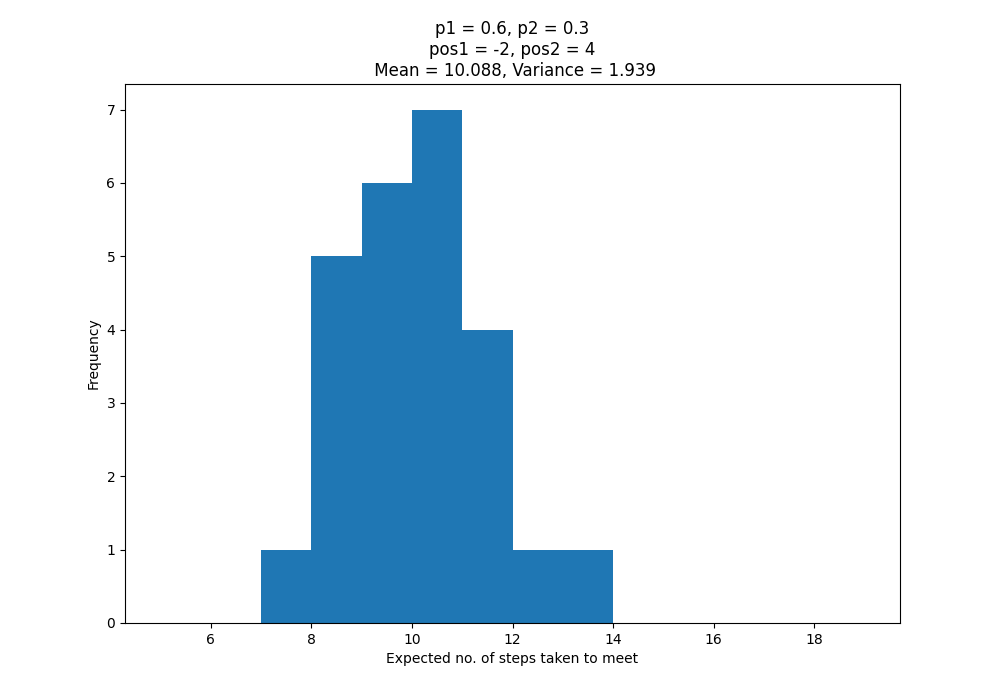
\includegraphics[scale = 0.5]{Q1_histograms/1.3/Q1.3 _p1 = 0.6_p2 = 0.3_pos1 = -2_pos2 = 4.png}
\end{center}

The above histogram shows that the expected number of steps to meet for two objects follows a normal distribution of mean $10.09$ and variance $1.94$ when they begin 6 steps apart with the given probabilities. \\
\begin{center}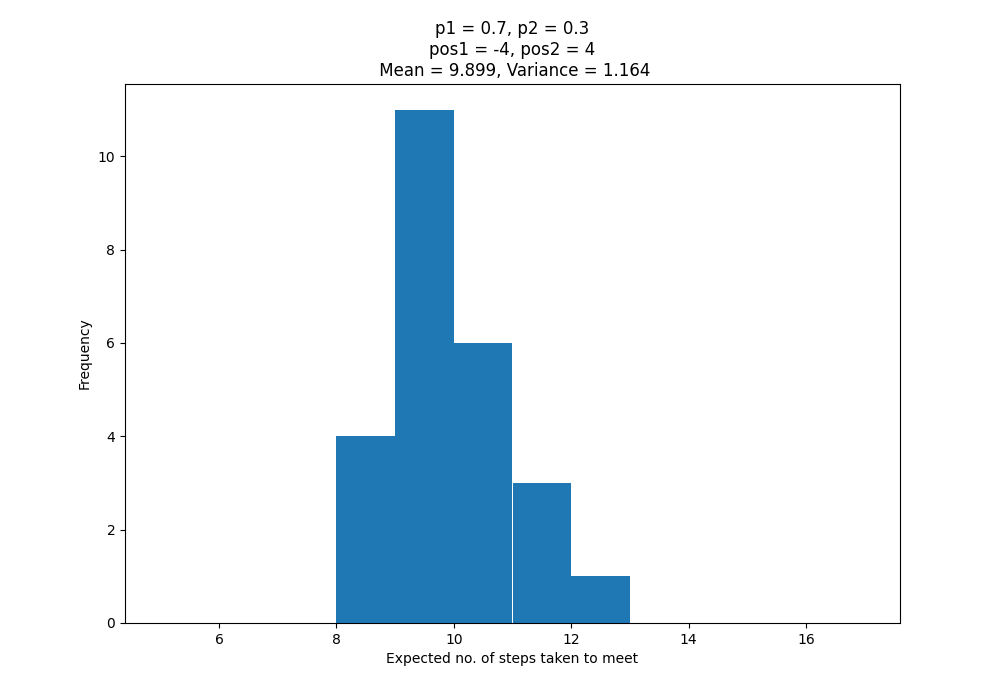
\includegraphics[scale = 0.5]{Q1_histograms/1.3/Q1.3 _p1 = 0.7_p2 = 0.3_pos1 = -4_pos2 = 4.png}\end{center}
The above histogram shows that the expected number of steps to meet for two objects follows a normal distribution of mean $9.90$ and variance $1.16$ when they begin 8 steps apart with the given probabilities. \\

% ------------------------------------------------- 5 -------------------------------------------------------------------
\pagebreak
\section*{Q5: Hypothesis Testing}
\subsection*{5.1}
\textbf{This question requires us to use hypothesis testing to determine whether the null hypothesis that a coin is fair is true or not. }\\
The following function implements the simulation of a fair coin:
\lstinputlisting[firstline=11,lastline=13,language=python]{q5.py}
This function then uses the above function to simulate 10 coin tosses 100 times and finds the expected number of times the null hypothesis is rejected for each iteration:
\lstinputlisting[firstline=15,lastline=36, language=python]{q5.py}
Histogram of expected values:
\begin{center}
  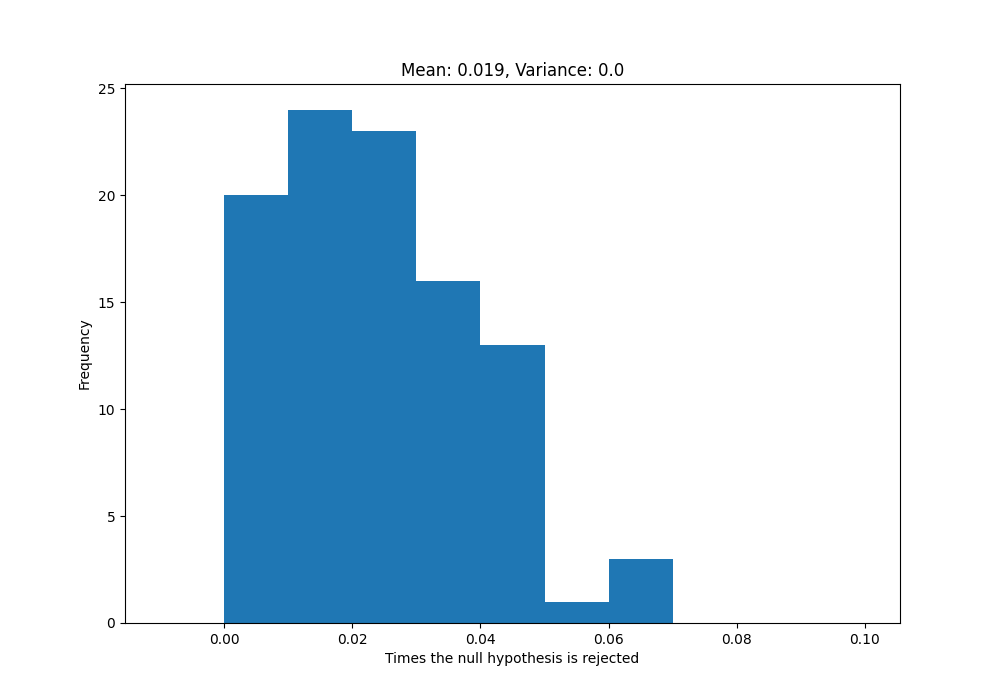
\includegraphics[scale = 0.5]{Q5_histograms/Q5.1.png}
\end{center}
Probability we will reject the null hypothesis even though it is true:\\
\emph{Simulation-wise}: According to the mean of the expected values, the probability is $2.3\%$.\\
\emph{Mathematically}: We reject the null hypothesis if the probability of the outcomes is below the threshold. Since the probability of the outcomes being accepted is 0.95 and the probability of them being rejected is 0.05, the probability that we reject the null hypothesis even though it is true is also 0.05 which is equal to the threshold.

\subsection*{5.2.1}
\textbf{This question requires us to use hypothesis testing to determine the validity of the null hypothesis that the mean length of fish in a lake is 23.}\\
The following function conducts a single hypothesis test by taking a sample of $30$ fish and calculating the mean and standard deviation of their lengths to check the following condition to accept or reject the null hypothesis:
\[P(|S - u_0| \geq a) < 0.05\]
The function returns $1$ if the hypothesis is rejected, and $0$ if it is accepted.
\lstinputlisting[firstline=42,lastline=54,language=python]{q5.py}
The following function performs 50 experiments and uses the average of their outcome to calculate a single expected value. It repeats this for 100 iterations and plots a histogram of the expected values.
\lstinputlisting[firstline=57,lastline=73,language=python]{q5.py}
Histogram of expected values of the null hypothesis being rejected:
\begin{center}
  
\includegraphics[scale = 0.5]{Q5_histograms/Q5.2.1.png}
\end{center}
The histogram follows a normal disttribution with mean 0.951 and variance 0.001. According to this, the null hypothesis is rejected $95\%$ of the times so it is false. A single hypothesis test may have been sufficient to accept or reject the null hypothesis as the variance is very low.

\subsection*{5.2.2}
The following function calls the \texttt{hypothesis\_test()} function defined in $5.2.1$ using the same value for the population mean $u_0$ $(23)$ but passing a value of 70 for the sample size $n$. It then performs 50 experiments and uses the average of their outcome to calculate a single expected value. It repeats this for 100 iterations and plots a histogram of the expected values.
\lstinputlisting[firstline=77,lastline=92,language=python]{q5.py}
Histogram of expected values of the null hypothesis being rejected:
\begin{center}
  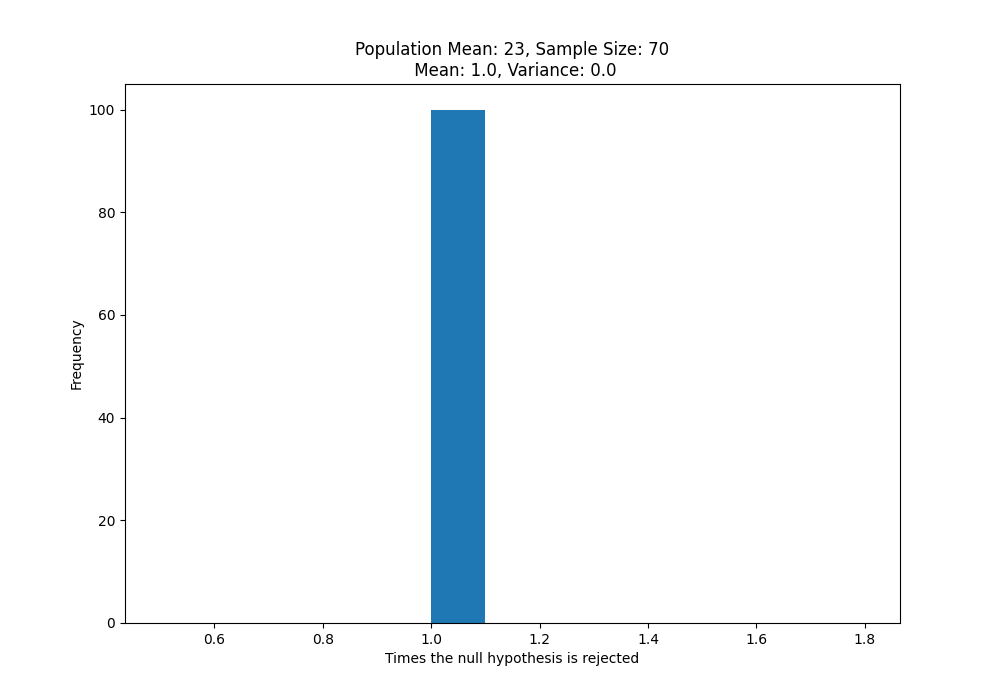
\includegraphics[scale = 0.5]{Q5_histograms/Q5.2.2.png}
\end{center}
Increasing the value of $n$ made the variance become $0$ where it was previously 0.001. In other words, the null hypothesis is rejected $100\%$ of the times. A single hypothesis test may have been sufficient to reject the null hypothesis in this case as there is no variance in the outcome.

\subsection*{5.2.3}
\textbf{Determining the least value of $n$ to ensure that the null hypothesis is not wrongly rejected more than 10 percent of the time using simulations.}\\ 

The following is a function that returns the length of a fish following a normal distribution with mean 23 and standard deviation 3.
\lstinputlisting[firstline=99,lastline=100,language=python]{q5.py}

In order to calculate the expected number of times the null hypothesis is rejected, we use the following function which takes in the value of the population mean $u_0$ and sample size $n$ and uses the \texttt{my\_fish()} function defined above to create the sample for the test. It then conducts the test itself the same way as the previous parts but with a threshold of 0.1.
\lstinputlisting[firstline=102,lastline=114,language=python]{q5.py}

We then use the following function which calls the \texttt{testing()} function, performs 50 experiments and uses the average of their outcome to calculate a single expected value. It repeats this for 100 iterations and plots a histogram of the expected values.
\lstinputlisting[firstline=116,lastline=132,language=python]{q5.py}
\pagebreak
Conducting simulations with various values of $n$, we achieve the above histograms.
\begin{figure}
  \centering
  \mbox{\subfigure{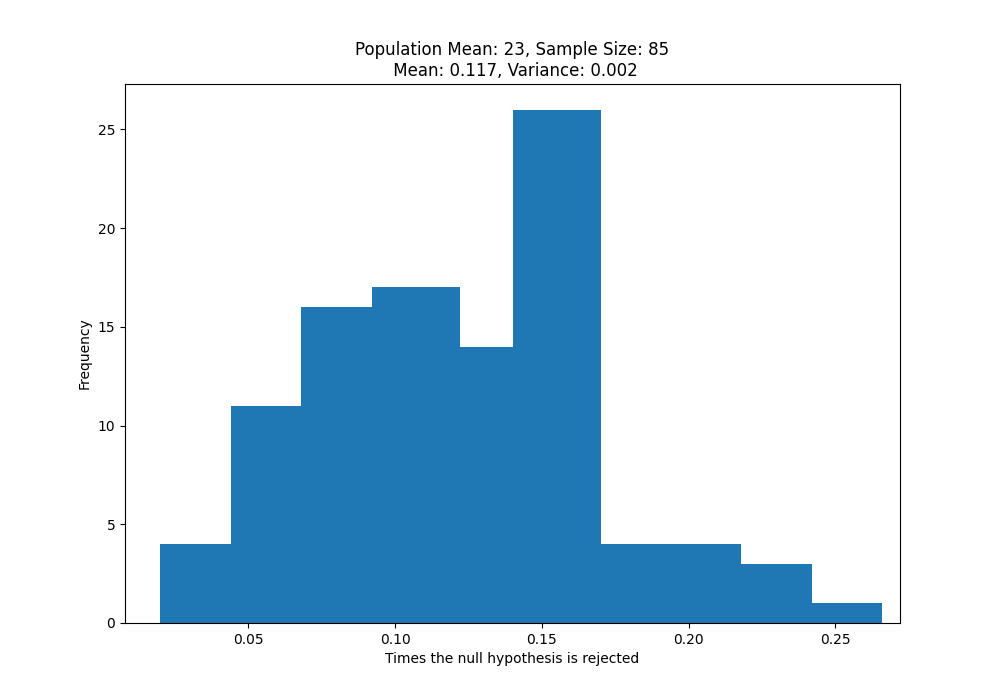
\includegraphics[scale = 0.35]{Q5_histograms/Q5.2.3_85.png}}\quad
  \subfigure{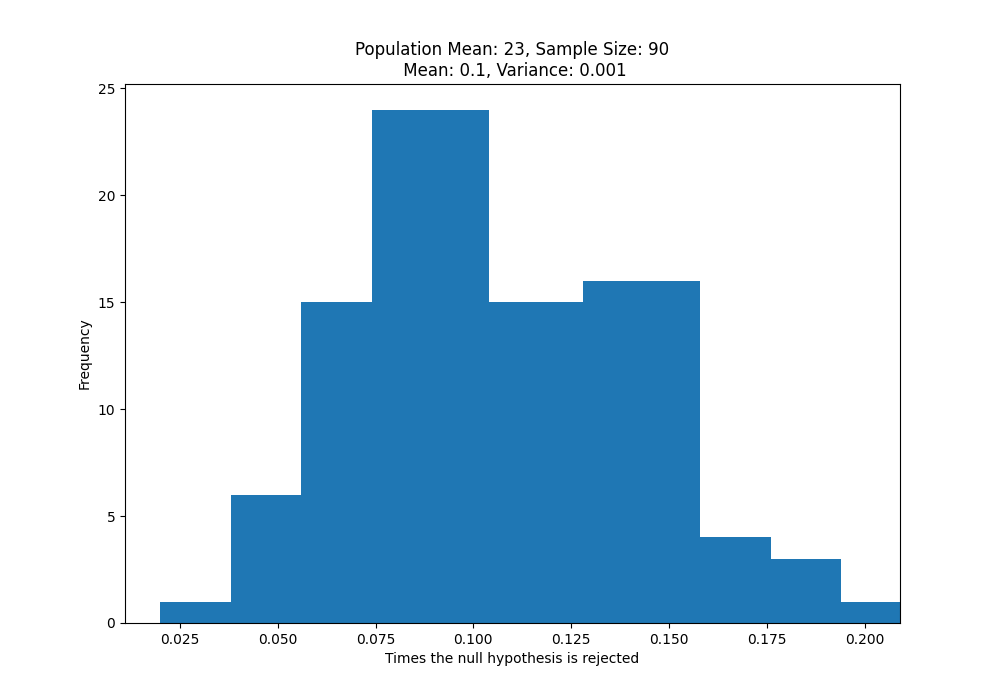
\includegraphics[scale = 0.35]{Q5_histograms/Q5.2.3_90.png}}}
\end{figure}
\begin{figure}
  \centering
  \mbox{\subfigure{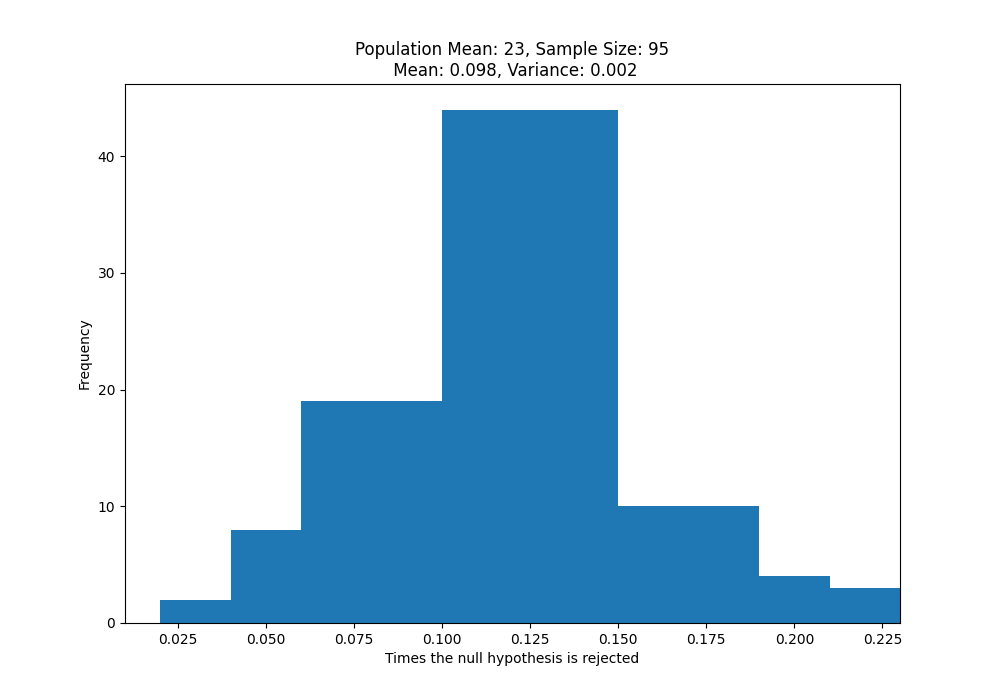
\includegraphics[scale = 0.35]{Q5_histograms/Q5.2.3_95(1).png}}\quad
  \subfigure{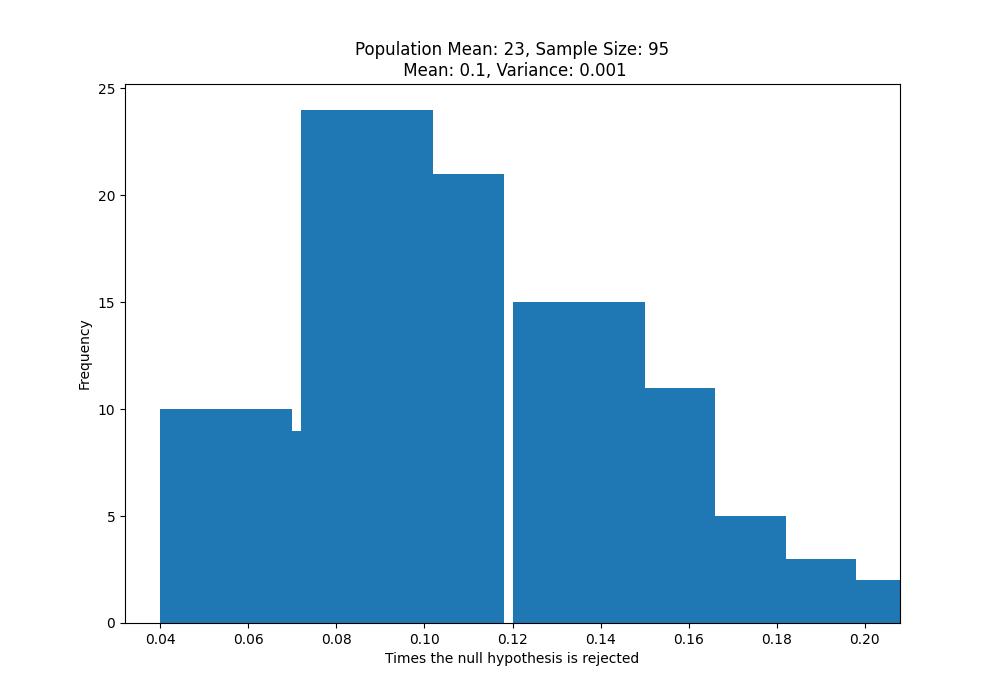
\includegraphics[scale = 0.35]{Q5_histograms/Q5.2.3_95(10).png}}}
\end{figure}
In order to determine the least value of $n$ to ensure that the null hypothesis is not wrongly rejected more than 10 percent of the times, we want a value of $n$ that gives a mean of 0.1. According to the simulations, the value of $n$ satisfying this condition is \textbf{90}. 

\end{document} 